\documentclass{presentation}

\usepackage{tikz}

% some details about the cover page
\title[slide $\text{\insertframenumber}$]{Efficient Algorithm}
\subtitle{Jump points}
\author{Rademacher, Loka}
\date{\today}
\institute{
    Department of Computer Science \\
    University of Bonn
}

\begin{document}


\begin{frame}
    \titlepage
\end{frame}



\begin{frame}{Contents}
    \begin{itemize}
        \item Path finding on grid graphs
        \item A Star Search ($A^\star$)
        \item Jump Point Search ($JPS$)
        \item Jump Point Search Improvements ($JPS^+$)
        \item Bounding Boxes ($BB$)
        \item Defined goal
    \end{itemize}
\end{frame}



\begin{frame}
    \bigbox{Path finding on grid graphs}
\end{frame}

\begin{frame}{Problem definition}
	\begin{minipage}{0.3\textwidth}

	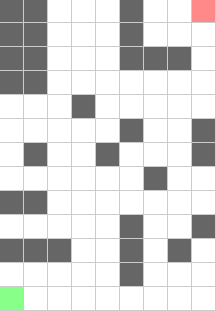
\includegraphics[width=\textwidth]{figures/gridgraph.png}
	
	\end{minipage}%
	\hfill%
	\begin{minipage}{0.6\textwidth}
	

	\begin{itemize}
		\item 4-tuple $(G, s, g, h)$:
		\pause
		\begin{itemize}
		\item[$\tikz{\path[draw=black,fill=white] (0,0) rectangle (2mm,2mm);}$] Euclidean grid graph $G$
		\item[$\tikz{\path[draw=black,fill=white!60!green] (0,0) rectangle (2mm,2mm);}$] start node $s$
		\item[$\tikz{\path[draw=black,fill=white!60!red] (0,0) rectangle (2mm,2mm);}$] goal node $g$
		\item[$\tikz{\path[draw=black,fill=gray] (0,0) rectangle (2mm,2mm);}$] $\not\in G$ obstacle
		\pause
		\item[$\rightarrow$] edge costs $1$
		\item[$\nearrow$] edge costs $\sqrt{2}$
		\pause
		\item[$h$:] a heuristic function
		\end{itemize}
	\end{itemize}
	
	\end{minipage}
	
	\hspace{3cm}
	
	\pause
	\begin{center}
		Goal: shortest path from $s$ to $g$ over $G$
	\end{center}

\end{frame}


\begin{frame}{Heuristic Function $h$}
	\begin{minipage}{0.3\textwidth}
		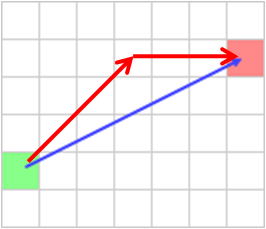
\includegraphics[width=\textwidth]{figures/heuristic.png}
	\end{minipage}%
	\hfill%
	\begin{minipage}{0.6\textwidth}
		\begin{itemize}
		\item $h(\tikz{\path[draw=black,fill=white!60!green] (0,0) rectangle (2mm,2mm);},\tikz{\path[draw=black,fill=white!60!red] (0,0) rectangle (2mm,2mm);})\leq min_{path}(\tikz{\path[draw=black,fill=white!60!green] (0,0) rectangle (2mm,2mm);},\tikz{\path[draw=black,fill=white!60!red] (0,0) rectangle (2mm,2mm);})$
		\pause
		\item e.g.:\\ $h(\tikz{\path[draw=black,fill=white!60!green] (0,0) rectangle (2mm,2mm);},\tikz{\path[draw=black,fill=white!60!red] (0,0) rectangle (2mm,2mm);}) = dist_{euklid}(\tikz{\path[draw=black,fill=white!60!green] (0,0) rectangle (2mm,2mm);},\tikz{\path[draw=black,fill=white!60!red] (0,0) rectangle (2mm,2mm);})$
		\begin{itemize}
			\item $\sqrt{27} \leq 3+3\cdot\sqrt{2}$
		\end{itemize}
		\end{itemize}
	\end{minipage}
\end{frame}

\begin{frame}
    \bigbox{A Star search ($A^\star$)}
\end{frame}



\begin{frame}
    \bigbox{Jump Point Search ($JPS$)}
\end{frame}



\begin{frame}
    \bigbox{Jump Point Search Improvements ($JPS^+$)}
\end{frame}



\begin{frame}
    \bigbox{Bounding Boxes ($BB$)}
\end{frame}



\begin{frame}
    \bigbox{Defined goal}
\end{frame}



\begin{frame}
    \bigbox{Thanks for attention!}
\end{frame}


\end{document}
